%%%%%%%%%%%%%%%%%%%%%%%%%%%%%%%%%%%%%%%%%
% a0poster Landscape Poster
% LaTeX Template
% Version 1.0 (22/06/13)
%
% The a0poster class was created by:
% Gerlinde Kettl and Matthias Weiser (tex@kettl.de)
%
% This template has been downloaded from:
% http://www.LaTeXTemplates.com
%
% License:
% CC BY-NC-SA 3.0 (http://creativecommons.org/licenses/by-nc-sa/3.0/)
%
%%%%%%%%%%%%%%%%%%%%%%%%%%%%%%%%%%%%%%%%%

%-------------------------------------------------------------------------------
%	PACKAGES AND OTHER DOCUMENT CONFIGURATIONS
%-------------------------------------------------------------------------------

\documentclass[a0, landscape]{a0poster}

\usepackage{multicol} % This is so we can have multiple columns of text side-by-side
\columnsep=100pt % This is the amount of white space between the columns in the poster
\columnseprule=3pt % This is the thickness of the black line between the columns in the poster

\usepackage[svgnames]{xcolor} % Specify colors by their 'svgnames', for a full list of all colors available see here: http://www.latextemplates.com/svgnames-colors

%\usepackage{times} % Use the times font
% \usepackage{palatino} % Uncomment to use the Palatino font
\usepackage{fontspec}
\setmainfont{Latin Modern Sans}

\usepackage{graphicx} % Required for including images
\graphicspath{{figures/}} % Location of the graphics files
\usepackage{booktabs} % Top and bottom rules for table
\usepackage[font=small,labelfont=bf]{caption} % Required for specifying captions to tables and figures
\usepackage{amsfonts, amsmath, amsthm, amssymb} % For math fonts, symbols and environments
\usepackage{wrapfig} % Allows wrapping text around tables and figures

\usepackage{listings}
\usepackage{color}

\definecolor{dkgreen}{rgb}{0,0.6,0}
\definecolor{gray}{rgb}{0.5,0.5,0.5}
\definecolor{mauve}{rgb}{0.58,0,0.82}

\lstset{
  %frame=tb,
  language=Python,
  aboveskip=2mm,
  belowskip=0mm,
  showstringspaces=false,
  columns=flexible,
  basicstyle={\small\ttfamily},
  numbers=none,
  numberstyle=\tiny\color{gray},
  keywordstyle=\color{blue},
  commentstyle=\color{dkgreen},
  stringstyle=\color{mauve},
  breaklines=true,
  breakatwhitespace=true,
  tabsize=3,
  framexleftmargin=15pt
  }


\begin{document}

%----------------------------------------------------------------------------------------
%	POSTER HEADER
%----------------------------------------------------------------------------------------

% The header is divided into three boxes:
% The first is 55% wide and houses the title, subtitle, names and university/organization
% The second is 25% wide and houses contact information
% The third is 19% wide and houses a logo for your university/organization or a photo of you
% The widths of these boxes can be easily edited to accommodate your content as you see fit

\begin{minipage}[b]{0.60\linewidth}
\Huge \color{NavyBlue} \textbf{GPU-accelerated diffusion MRI tractography in DIPY} \color{Black} \\ % Poster title
{\LARGE Mauro Bisson\textsuperscript{1}, Josh Romero\textsuperscript{1}, Thorsten Kurth\textsuperscript{1}, Massimiliano Fatica\textsuperscript{1}, Pablo F. Damasceno\textsuperscript{2}, Xihe Xie\textsuperscript{2},\\ Adam Richie-Halford\textsuperscript{3}, Serge Koudoro\textsuperscript{4}, Eleftherios Garyfallidis\textsuperscript{4}, \&  Ariel Rokem \textsuperscript{3}}\\ % Author(s)
\Large 1. NVIDIA, 2. University of California, San Francisco, 3. University of Washington, 4. Indiana University  \\ % University/organization
\Large Contact: \texttt{arokem@uw.edu}
\end{minipage}
%
%\begin{minipage}[b]{0.25\linewidth}
%\color{DarkSlateGray}\Large \textbf{Contact Information:}\\
%Department Name\\ % Address
%University Name\\
%123 Broadway, State, Country\\\\
%Phone: +1 (000) 111 1111\\ % Phone number
%Email: \texttt{john@LaTeXTemplates.com}\\ % Email address
%\end{minipage}
%
\begin{minipage}[b]{0.4\linewidth}

\includegraphics[height=5cm]{UWlogo.png}

\includegraphics[height=5cm]{iulogo.jpeg}

\includegraphics[height=4cm]{Nvidia_logo.png}

\includegraphics[height=5cm]{UCSFlogo.png}


\end{minipage}

\vspace{0.5cm} % A bit of extra whitespace between the header and poster content

%----------------------------------------------------------------------------------------

\begin{multicols}{3} % This is how many columns your poster will be broken into, a poster with many figures may benefit from less columns whereas a text-heavy poster benefits from more

%----------------------------------------------------------------------------%	Introduction
%----------------------------------------------------------------------------

\section*{Introduction}

The white matter of the brain contains the axons of long-range connections between distant brain regions. The integration and coordination of brain activity through these connections are important for information processing and for brain health. Diffusion-weighted MRI (dMRI) and computational tractography provide non-invasive in vivo estimates of the trajectories of these brain connections.

This is done by estimating the directions of diffusion in every voxel of measurement, and by propagating streamlines through the volume based on the peaks in the distribution of diffusion directions. The resulting tractograms are important in research that uses dMRI to measure individual differences in brain connections. They are also important in clinical use-cases, where invasive procedures are guided by these estimates, aiming to avoid disconnections of crucial brain pathways. However, a major barrier to progress in the use of these methods is that tractography can be a computationally-intensive processing step.

\vspace{0.5em}
\noindent\textbf{\underline{Challenge}: Even when highly-efficient CPU-based implementations are provided in open-source software, these can take hours to process millions of streamlines in an individual brain.}
\vspace{0.5em}

\noindent\textbf{\underline{Solution}: By taking advantage of the massively parallel architecture of graphical processing units (GPU) and the implementations of very fast basic computational operations, GPU-based computing can be used to accelerate many scientific use-cases.}
\vspace{0.5em}

\subsection*{DIPY: Software framework for analysis of dMRI \cite{Garyfallidis2014FrontNeuroinf}}

\begin{minipage}[b]{1\linewidth}
\begin{minipage}[b]{0.5\linewidth}
    \begin{itemize}
    \item Open-source
    \item Community-developed
    \item Contains implementations of methods for
    \begin{itemize}
        \item Diffusion reconstruction
        \item Tractography
        \item Bundle recognition and streamline clustering
        \item Image registration and segmentation
    \end{itemize}
    \end{itemize}
\end{minipage}
\begin{minipage}[b]{0.65\linewidth}
    \includegraphics[height=5cm]{dipy-logo.png} \\
    \begin{centering}
    \LARGE \texttt{https://dipy.org}
    \end{centering}
\end{minipage}
\end{minipage}

\subsection*{GPU tractography}

\noindent Relying on the DIPY implementation of residual bootstrap tractography \cite{berman2008probabilistic}, we implemented a multi-GPU parallelizable version constructed on NVIDIA’s CUDA application programming interface (API).  The API of the GPU version is compatible with the one implemented in DIPY, enabling direct comparisons and interoperability.

\section*{Methods}


\subsection*{Data}
\begin{itemize}
\item HARDI acquisition with 2x2x2 $mm^3$ isotropic voxels, 150 b=1,000~$\frac{s}{mm^2}$ volumes and 10 b0 volumes \cite{rokem2015evaluating}.

\item Super-Resolution Hybrid Diffusion Imaging  (HYDI), with an effective resolution of 0.625x0.625x0.625 $mm^3$ isotropic voxels, b=500, 800, 1600, 2600~$\frac{s}{mm^2}$, in 134 diffusion directions, and 8 b0 volumes \cite{elsaidsuper}.
\end{itemize}

\subsection*{Experiments}

\noindent Experiments to profile the performance of the algorithm were conducted using an AWS p3.16xlarge instance with 8 NVIDIA Tesla V100 Graphical Processing Units and 488 GB RAM. For comparison, CPU code was run on an AWS x1e.4xlarge with 488 GB RAM. In both cases, 27 tracking seeds were placed in each voxel in the white matter to initialize tracking.

\vfill
\columnbreak
\color{Navy}

%----------------------------------------------------------------------------%	RESULTS
%----------------------------------------------------------------------------


\section*{Performance benchmark}

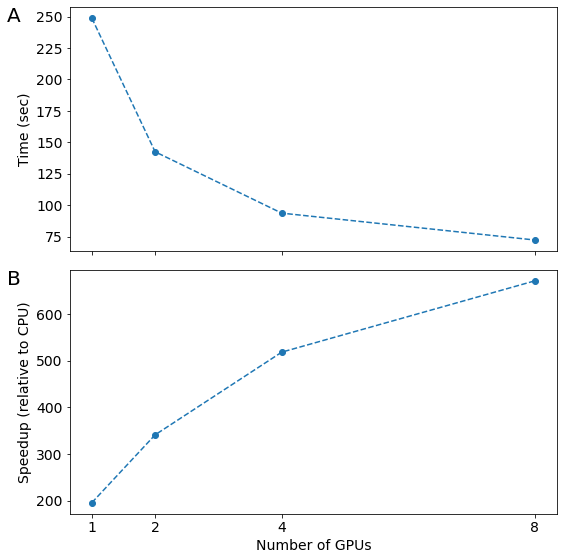
\includegraphics[width=0.8\linewidth]{benchmark.png}

For the same task (HARDI data, 27 seeds per WM voxel) tractography duration decreases with the number of GPUs available. Speedup relative to CPU ranges from approximately 200-fold, with one GPU to almost 700-fold with 8 GPUs.

\section*{HYDI tractography}

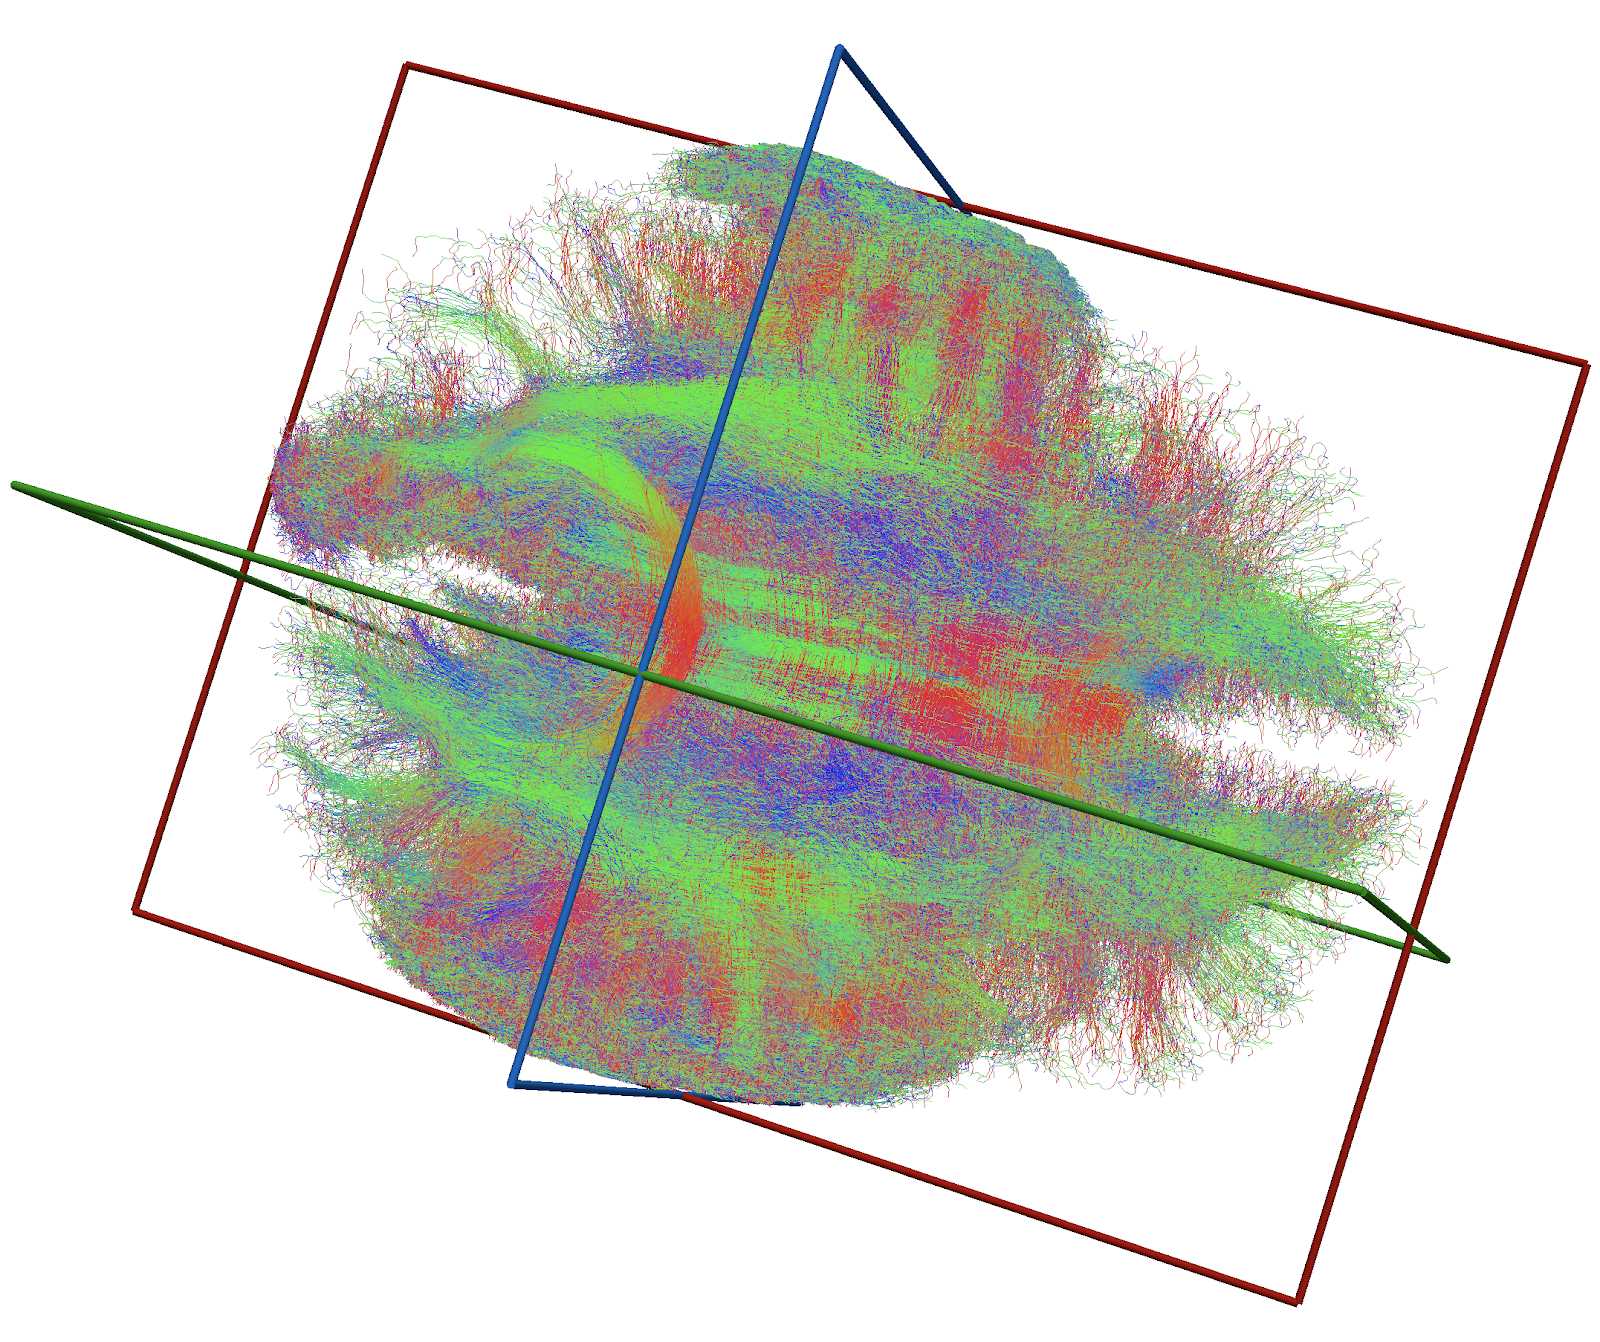
\includegraphics[width=0.8\linewidth]{hydi-tractography.png}

GPU-accelerated tractography of high-resolution data, acquired at 0.625 $mm^3$  effective resolution. This is a small subset sampled randomly for visualization purposes: approximately 8M streamlines of the 150M streamlines tracked.


\columnbreak

\color{SaddleBrown} % SaddleBrown color for the conclusions to make them stand out

\section*{Conclusions}
\large
\begin{itemize}

\item GPU-accelerated tractography algorithms that leverage the methods implemented in the DIPY open-source software project accelerate tractography by at least 200-fold, enabling applications to clinical data, as well as very large datasets.

\item Open source software is available at: \\ \texttt{https://github.com/dipy/GPUStreamlines}

\item Docker image available at: \\ \texttt{docker pull ghcr.io/dipy/gpustreamlines:latest}

\small

docker run --gpus=all -v ${PWD}:/opt/exec/output:rw -it ghcr.io/dipy/gpustreamlines:latest \
 python run_dipy_gpu_hardi.py --chunk-size 100000 --ngpus 1 --output-prefix output/hardi_gpu_full --use-fast-write

 docker run --gpus=all -v ${PWD}:/opt/exec/output:rw -it ghcr.io/dipy/gpustreamlines:latest \
 ./merge_trk.sh -o output/hardi_tracks.trk output/hardi_gpu_full*

\end{itemize}

\color{DarkSlateGray} % Set the color back to DarkSlateGray for the rest of the content

%---------------------------------------------------------------------------	REFERENCES
%----------------------------------------------------------------------------

\nocite{*} % Print all references regardless of whether they were cited in the poster or not
\bibliographystyle{plain} % Plain referencing style
\footnotesize \bibliography{poster} % Use the example bibliography file sample.bib

%----------------------------------------------------------------------------%	ACKNOWLEDGEMENTS
%----------------------------------------------------------------------------
\subsection*{Acknowledgements} \footnotesize


\includegraphics[height=2.6cm]{NIBIB.png}

\includegraphics[height=2.6cm]{nimh-logo.png} \\
\includegraphics[height=2.6cm]{SloanLogo.png}
\includegraphics[height=2.6cm]{MooreFdn.png}
\includegraphics[height=2.6cm]{eSciencelogo.png}
%----------------------------------------------------------------------------

\end{multicols}
\end{document}
